\chapter{Experiments and Results}
\label{ch:results}

For each result, the value, the denominator and the permitted claim boundary are
given. All numbers are read from recorded artifacts.

\section{Coverage of Acceptance Conditions and Evidence Status}
\label{sec:res-gates}

Table~\ref{tab:gates} places the official acceptance conditions (human labels,
target hardware, a completed study) next to the automatic evidence of the final
stage; the automatic evidence does not replace the official conditions.

\begin{table}[ht]
\centering
\caption{Official acceptance conditions and the final automatic evidence}
\label{tab:gates}
\small
\begin{tabular}{L{5.0cm}cL{5.2cm}}
\toprule
\textbf{Acceptance condition} & \textbf{Official} & \textbf{Final automatic evidence} \\
\midrule
Working Persian speech-to-speech prototype & sufficient & streaming system and loopback test \\
Final automatic semantic test & sufficient & -- \\
Audited 100--200 hour export & sufficient & -- \\
Data policy under a documented waiver & sufficient & -- \\
Source code licence & sufficient & -- \\
\midrule
Deployable direct model & negative & v7a: 6/9, unintelligible \\
Detector above 80\% & not human & simulation 0.933/0.880; browser 0.825/0.817 \\
Latency and memory on target hardware & not target hardware & 11.1~GiB; mean 372, 90th percentile 431 \\
Human study & pending & registered instrument \\
\bottomrule
\end{tabular}
\end{table}

\section{Dataset}
\label{sec:res-data}

Table~\ref{tab:corpus} shows the final characteristics. The 108.584 hours fall
within the range of R4, and the automatic integrity audit, including channel
order, hashing and group splits, passed without failure.

\begin{table}[ht]
\centering
\caption{Characteristics of the derived Persian conversational dataset}
\label{tab:corpus}
\small
\begin{tabular}{L{7.6cm}R{3.2cm}}
\toprule
\textbf{Indicator} & \textbf{Value} \\
\midrule
Caption inventory of the channels & 775.887 hours \\
Response pairs without reuse & 6,754 \\
Source audio hours of the pairs & 123.796 hours \\
Speakers / sessions & 407/162 \\
Exported stereo hours & 108.584 hours \\
Train / validation / test split & 6,419/131/204 \\
Group leakage / automatic audit failures & 0/0 \\
Automatic interaction-event candidates & 770 \\
Human-verified rows & 0 \\
\bottomrule
\end{tabular}
\end{table}

An independent automatic listener (Gemini, two passes, agreed labels only) on 300
available pairs heard another speaker start at 93.8\% of turn boundaries and
confirmed 75.7\% of the marked overlaps; the captions differ from its transcript
by a 15.9\% character error rate.

\claim{The interaction labels are automatic candidates and their verification is
automatic too. This dataset cannot be called human-labelled, and the source data
are not redistributable.}

\section{Cascade System: Mechanical Panel and Intelligibility}
\label{sec:res-cascade}

The validation panel is nine evenly spaced rows of the 131-row manifest. The row
indices were locked before running. The chain is the real recognition service,
the Qwen2.5-0.5B-Instruct responder and the real speech engine, with the audited
user channel one as input. This panel measures the mechanics of the chain, not the
semantic quality of Qwen3-4B. The result is in Table~\ref{tab:cascade-panel}.

\begin{table}[ht]
\centering
\caption{Result of the fixed validation panel of the cascade}
\label{tab:cascade-panel}
\small
\begin{tabular}{L{7.8cm}R{3.0cm}}
\toprule
\textbf{Indicator} & \textbf{Value} \\
\midrule
Text responder of the panel & Qwen2.5-0.5B \\
Rows passing every condition & 9/9 \\
Rows with a rule-based fallback reply & 0/9 \\
Minimum Persian-character share in transcript and reply & 1.000 \\
Non-silent audio replies & 9/9 \\
Minimum RMS of the reply audio & 0.133529 \\
Median / maximum full generation time (ms) & 5584.7/13270.2 \\
Final-test rows used & 0 \\
\bottomrule
\end{tabular}
\end{table}

The median, 95th percentile and maximum transcript lengths were 445, 3977.8 and
5031 characters. The descriptive Pearson correlation between transcript length
and full generation time is 0.885; the longest transcript and the slowest turn
were both row 32. The time column is the duration of full reply generation, not
first-audio latency.

Re-recognition of the same nine outputs, with the reply text as reference, gave a
micro-aggregated character error rate of 7.14\% (47/658) and a word error rate of
30.41\% (52/171). No row had an exact word or character match.
Figure~\ref{fig:cascade} shows both axes.

\begin{figure}[ht]
\centering
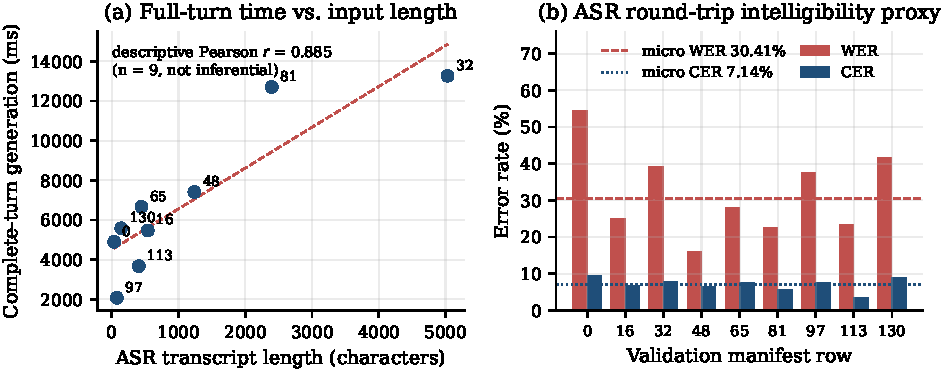
\includegraphics[width=0.96\textwidth]{figs/cascade_panel.pdf}
\caption{(a) Full generation time against transcript length for the nine panel
         rows. (b) Word and character error rates of re-recognizing the same nine
         outputs.}
\label{fig:cascade}
\end{figure}

\claim{The mechanical result is out-of-sample with the Qwen2.5-0.5B responder and
is not generalized to Qwen3-4B. Nine rows are not enough for population
generalization. Full generation time is not the $T_{\text{first\_audio}}$ measure
and does not meet the 500 ms condition. Re-recognition does not prove human
intelligibility or naturalness.}

\section{Automatic Semantic Test}
\label{sec:res-semantic}

The qualification stage on seven unused validation rows passed every condition:
42/42 valid calls, relevance 3.857 versus 1.000, coherence 3.571, paired wins 6/7,
and relevance of at least two in 100\% of rows. Only after this pass was the final
test opened, once.

The final test ran on 40 rows of the 204-row manifest from five held-out
sessions. Three blind arms: the locked Qwen2.5-0.5B baseline, the Qwen3-4B
candidate with prompt v2, and the automatically aligned next-turn reference. The
judge was Qwen3.8-27B-FP8 at temperature zero with two repetitions per row.
Table~\ref{tab:semantic} shows the result and Table~\ref{tab:semantic-gates} the
passing of all seven predefined conditions.

\begin{table}[ht]
\centering
\caption{Result of the final automatic semantic test on 40 group-disjoint rows}
\label{tab:semantic}
\small
\begin{tabular}{L{6.8cm}R{4.2cm}}
\toprule
\textbf{Indicator} & \textbf{Value} \\
\midrule
Valid / expected judge calls & 240/240 \\
Judge repetition agreement & 1.00 \\
Mean relevance candidate / baseline / reference & 3.150/1.425/0.950 \\
Mean coherence candidate / baseline & 3.325/1.525 \\
Relevance / coherence gain over the baseline & +1.725/+1.800 \\
Paired relevance wins & 27/40 (67.5\%) \\
Relevance of at least two & 35/40 (87.5\%) \\
Candidate generation retries / invalid audio & 0/0 \\
\bottomrule
\end{tabular}
\end{table}

\begin{table}[ht]
\centering
\caption{Predefined automatic conditions of the final test}
\label{tab:semantic-gates}
\small
\begin{tabular}{L{5.8cm}rrc}
\toprule
\textbf{Condition} & \textbf{Threshold} & \textbf{Observed} & \textbf{Status} \\
\midrule
Candidate mean relevance & $\ge$ 2.00 & 3.150 & met \\
Candidate mean coherence & $\ge$ 2.50 & 3.325 & met \\
Relevance gain & $\ge$ 0.50 & 1.725 & met \\
Coherence gain & $\ge$ 0 & 1.800 & met \\
Paired relevance win rate & $\ge$ 0.60 & 0.675 & met \\
Rate of relevance at least two & $\ge$ 0.70 & 0.875 & met \\
Full mechanical validity & 240/240 & 240/240 & met \\
\bottomrule
\end{tabular}
\end{table}

Figure~\ref{fig:semantic} shows the means and the distribution of scores. The low
score of the aligned reference shows that ``saying the corpus's next turn'' is not
necessarily an appropriate reply to the user's utterance.

\begin{figure}[ht]
\centering
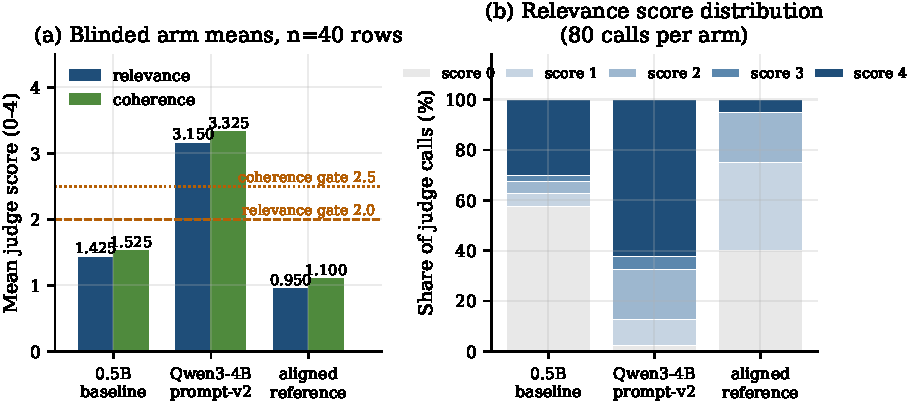
\includegraphics[width=0.96\textwidth]{figs/semantic_final_test.pdf}
\caption{(a) Mean relevance and coherence of the three blind arms.
         (b) Distribution of the relevance score over the 80 judge calls of each
         arm.}
\label{fig:semantic}
\end{figure}

A side LoRA experiment on the responder reduced the development loss by 31.18\%
but did not beat the baseline in the semantic evaluation and was not used in the
final system.

\claim{Passing seven automatic conditions does not mean perceptual quality or an
independent benchmark. The judge and the candidate are of the same family.}

\section{Component Re-Selection}
\label{sec:res-reselection}

All three components were compared again under new protocols.
\textbf{Recognition:} on 344 PSRB clips with human transcripts, Seamless was the
most accurate (character error rate 6.92\%) but, with a median of 671 ms, exceeded
the 150 ms budget; NeMo version 4, with 9.44\% and 58 ms, was the best candidate
within the budget and was retained (Whisper large-v3, Qwen3-ASR and Gemma~4 above
20\%). \textbf{Responder:} on a panel of 60 elderly requests and 60 natural turns,
no candidate reached the replacement threshold (+0.25 relevance) under both
judges. The judges disagree: under Gemini, Qwen3.5-4B and Gemma~4 with the elderly
prompt are about one point better than the deployed system (3.36 and 3.54 versus
2.38), but not under the Qwen judge (3.31 and 3.00 versus 3.29). The Qwen3.5-4B
configuration passed the pre-registered deployment qualification (memory
11.1~GiB, mean and 90th-percentile latency 345 and 398 ms, coherence after
interruption under both judges); its replacement depends on the preference of
the listening-study participants. \textbf{Voice:} of the six Persian Piper voices,
Mana remained the most intelligible to two automatic listeners, with a mean
character error rate of 5.82\%; ganji\_adabi was tied and had the best DNSMOS, and
both went to the listening study. ParsVoice-XTTS with the ManaTTS voice was on par
on a typical clip but broke about one clip in ten (mean error 13.55\%,
significantly worse), and its first streaming chunk took 307 ms; it did not enter
the study. The lab VITS model, even after inference optimization without
retraining (error from 9.89\% to 9.19\%, the highest DNSMOS), stayed significantly
worse than Mana and did not enter the study.

\section{Interruption Detection}
\label{sec:res-bargein}

The deployed controller was measured in a deployment simulation: the microphone
during playback, residual echo of the reply, background noise, a room response
and one real event (an interruption, a backchannel, noise or nothing). Six
development runs used only the training split: a duration-and-classifier
confirmation 0.687, the lexical confirmation 0.840, and with corrected
initialization of the double-talk detector and echo adaptation 0.920. The chosen
variant reached, once, on 600 test scenarios an accuracy of \textbf{0.933} and an
F1 of \textbf{0.880} (recall 0.98; wrong stops on backchannels 8.7\%, noise
9.3\% and no event 6.7\%), with a median of 120 ms from the acoustic onset to the
duck. The energy/pitch/MFCC classifier reached only an accuracy of 0.574 and an
F1 of 0.672 on 94 podcast test events with Gemini labels.

\claim{A simulated mixture built from real recordings, with automatic labels; not
a live user.}

\section{Direct Track}
\label{sec:res-moshi}

Table~\ref{tab:moshi-summary} summarizes the seven generations. The common
pattern: the loss decreases and the runtime condition is not met. The minimum
losses are not directly comparable across generations, because the window and the
evaluation set differ. For v6.2 and v7a the loss is in-sample.

\begin{table}[ht]
\centering
\caption{Summary of the seven generations of the direct track. ``Best run'' is the
         largest number of the nine rows passed among the checkpoints of that
         generation.}
\label{tab:moshi-summary}
\small
\begin{tabular}{lrrrrc}
\toprule
\textbf{Version} & \textbf{Window} & \textbf{Candidates} & \textbf{Minimum} &
\textbf{Best} & \textbf{Eligible} \\
 & \textbf{(s)} & & \textbf{loss} & \textbf{run} & \\
\midrule
v1   & 20  & 16 & 1.402 & 0/9 & no \\
v2   & 100 & 20 & 1.735 & 2/9 & no \\
v3   & 100 & 5  & 1.879 & 1/9 & no \\
v4   & 100 & 5  & 1.879 & 1/9 & no \\
v5   & 100 & 5  & 1.868 & 1/9 & no \\
v6.2 & 12  & 4  & 2.060 & 0/9 & no \\
v7a  & 12  & 4  & 1.264 & 6/9 & no \\
\bottomrule
\end{tabular}
\end{table}

In v6.2 the best text loss after step 50 is 0.550852, 32.20\% lower than the
0.812474 at step 50 and above the 30\% criterion; that is, the adapter has the
capacity to fit the target. Nevertheless all four checkpoints scored 0 of 9, and
in each checkpoint only one of the nine rows produced text and speech together.
Figure~\ref{fig:trials} sets these two axes against each other.

\begin{figure}[ht]
\centering
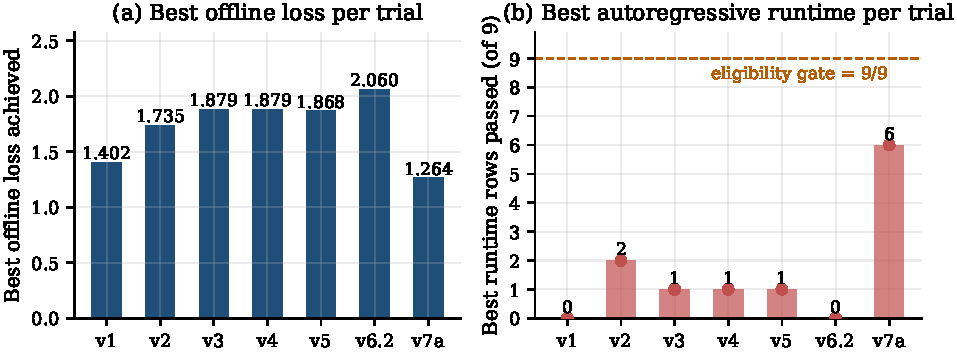
\includegraphics[width=0.96\textwidth]{figs/moshi_trials_summary.pdf}
\caption{(a) Best offline loss of each generation. (b) Largest number of rows
         passing the runtime panel, against the 9/9 condition.}
\label{fig:trials}
\end{figure}

\claim{No checkpoint is eligible for deployment. The statement ``Moshika was
successfully fine-tuned for Persian'' is false on this evidence.}

\textbf{Version seven.} With romanized text and word-by-word timing, the best
accepted count in the same capacity test reached 6/9 (controlled baseline 3/9),
and the server produced audible speech with text on 8 of 9 rows; but the 9/9
condition was not met and the generated speech was not intelligible to a Persian
recognizer (mean prefix error 0.88), so full training was not started. The
tokenizer bottleneck is real but not the only obstacle.

\textbf{Speech input.} Gemma~4, hearing the audio directly, scored 1.98 and 2.05
in relevance zero-shot and with the adapter, against 2.80 for the cascade; the
result is negative by the pre-registered rule. Removing recognition, even with the
same language model, lowered quality (2.49 versus 1.98) and saved only about 20 ms.
With the second judge (Gemini) the deployed system scored lowest (1.91) and the
speech-input path higher (2.18, and 2.52 with the adapter); the official result
with the first judge stays negative, and this disagreement between the judges is
reported. Gemma~4~12B understood Persian speech even worse than E4B.

\section{Latency, Memory and Browser Loopback}
\label{sec:res-unmet}

A headless browser ran the real client page with a fake microphone (recorded
utterances of 1--5 seconds). The language model server was limited to the memory
share of a 12 GB card: the peak GPU memory of the whole system was 11.1~GiB (at
H100 speed). With the speculative start after 96 ms of silence (chosen on
development utterances), no turn of the 201 turns of the main panel went
unanswered; the mean latency from end of speech to first audio was
\textbf{372}, the 90th percentile \textbf{431} and the maximum 491 ms (the first
run with 160 ms: 418, 487 and 537); with the browser's output latency, the 90th
percentile is 473. Simulated elderly speech: mean 382 and 90th percentile 446. In
120 turns with interruptions and backchannels, the decision accuracy was 0.825,
the F1 0.817, and the median time to duck from the detected onset 44 ms. In 30
scripted dialogues with a follow-up question over the reply, 24 of 27
interruptions stopped the reply, and the reply after an interruption was as
relevant as the reply to a normal turn under both judges. A semantic end-of-turn
gate (Smart Turn v3.2~\cite{smartturn2025}, an LLM judgement, a lexical rule and a
Smart Turn fine-tuned on Persian) lowered premature endpointing on development
utterances from 19.8\%, but no candidate delayed fewer than 13\% of genuine turn
ends (pre-registered limit 5\%); the deployed endpointer remained unchanged.

\claim{Automated loopback on an H100 without a human user or a physical audio
path; the proposal's criterion (mean and 90th percentile) and, on the main panel,
the every-turn reading are met.}

The small listening study (naturalness of two Piper voices and human speech,
three recorded dialogues, and a preference between the replies of two responders
that, by a pre-registered rule, decides on replacing the responder) is ready with a
registered protocol; its results are not yet available.

\section{Final Status of the Requirements}
\label{sec:res-requirements}

\begin{table}[ht]
\centering
\caption{Final status of the seven requirements of the project definition}
\label{tab:req-status}
\small
\begin{tabular}{cL{4.2cm}L{6.0cm}}
\toprule
\textbf{ID} & \textbf{Status} & \textbf{Supporting evidence} \\
\midrule
R1 & met (streaming cascade) & final semantic test; all 401 loopback turns answered \\
R2 & met in automated tests & interruptions 0.83/0.82 in the browser, 0.93/0.88 in simulation \\
R3 & met & mean 372 and 90th percentile 431; maximum 491 ms \\
R4 & met & 108.584 hours of audited export (automatic labels) \\
R5 & goal met by another method & lexical confirmation; acoustic classifier alone 0.574 \\
R6 & declared deviation & memory 11.1~GiB; speed on an H100 \\
R7 & awaiting results & registered instrument and protocol \\
\bottomrule
\end{tabular}
\end{table}

\claim{The evidence for R2, R3 and R5 is automated and on an H100; R4 has no human
labels; R5 was not met by the specified acoustic features alone.}

Of the four expected outputs, three have been produced and documented: the
streaming cascade prototype, documented source code, and the Persian
conversational dataset. Empirical findings on older adults can be reported once
the listening-study responses arrive.
